\section{J1640+2224}
\label{sec:J1640}

\subsection{Epoch-wise DM(t) correction}
\begin{center}
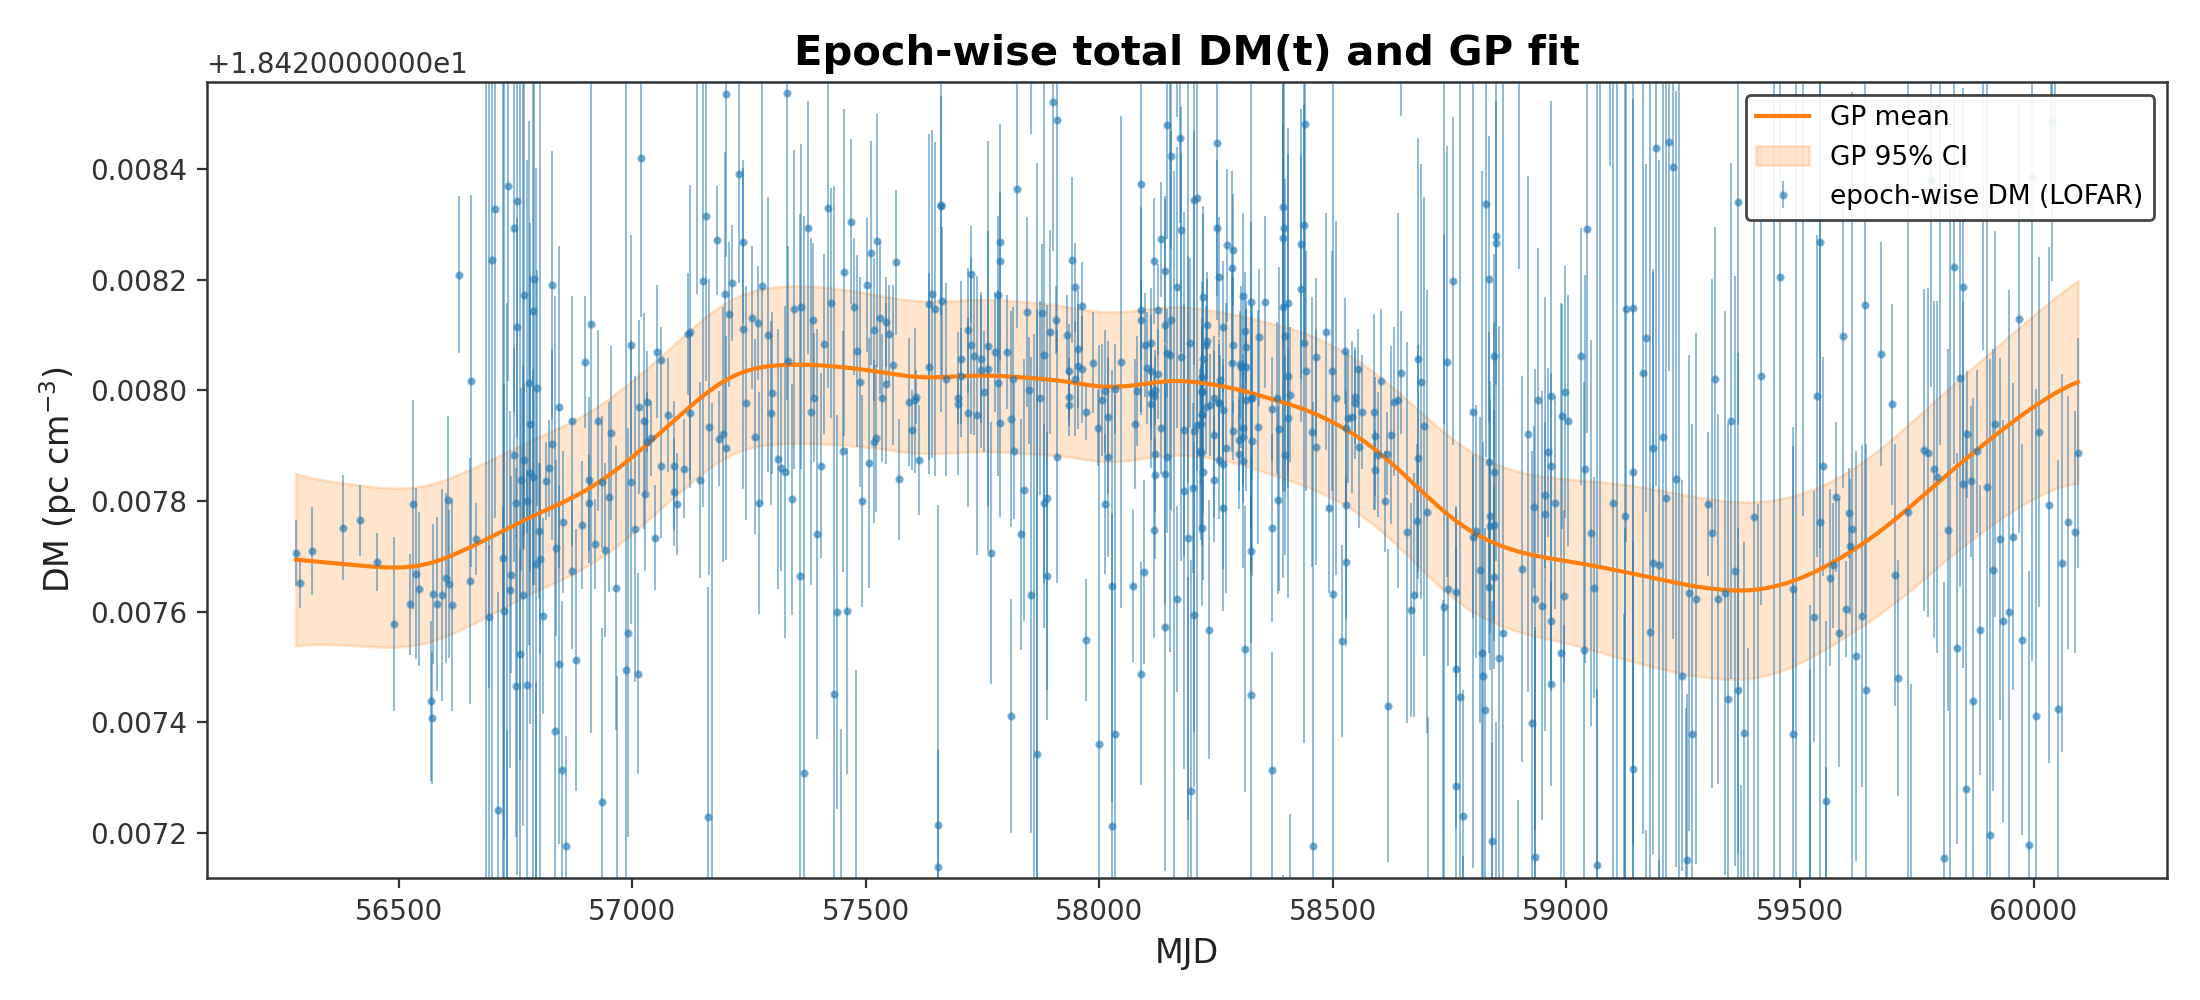
\includegraphics[width=0.8\textwidth]{../J1640+2224/dm_correction_out/dm_timeseries.png}
\end{center}

\subsection{Effect on residuals}
\begin{center}
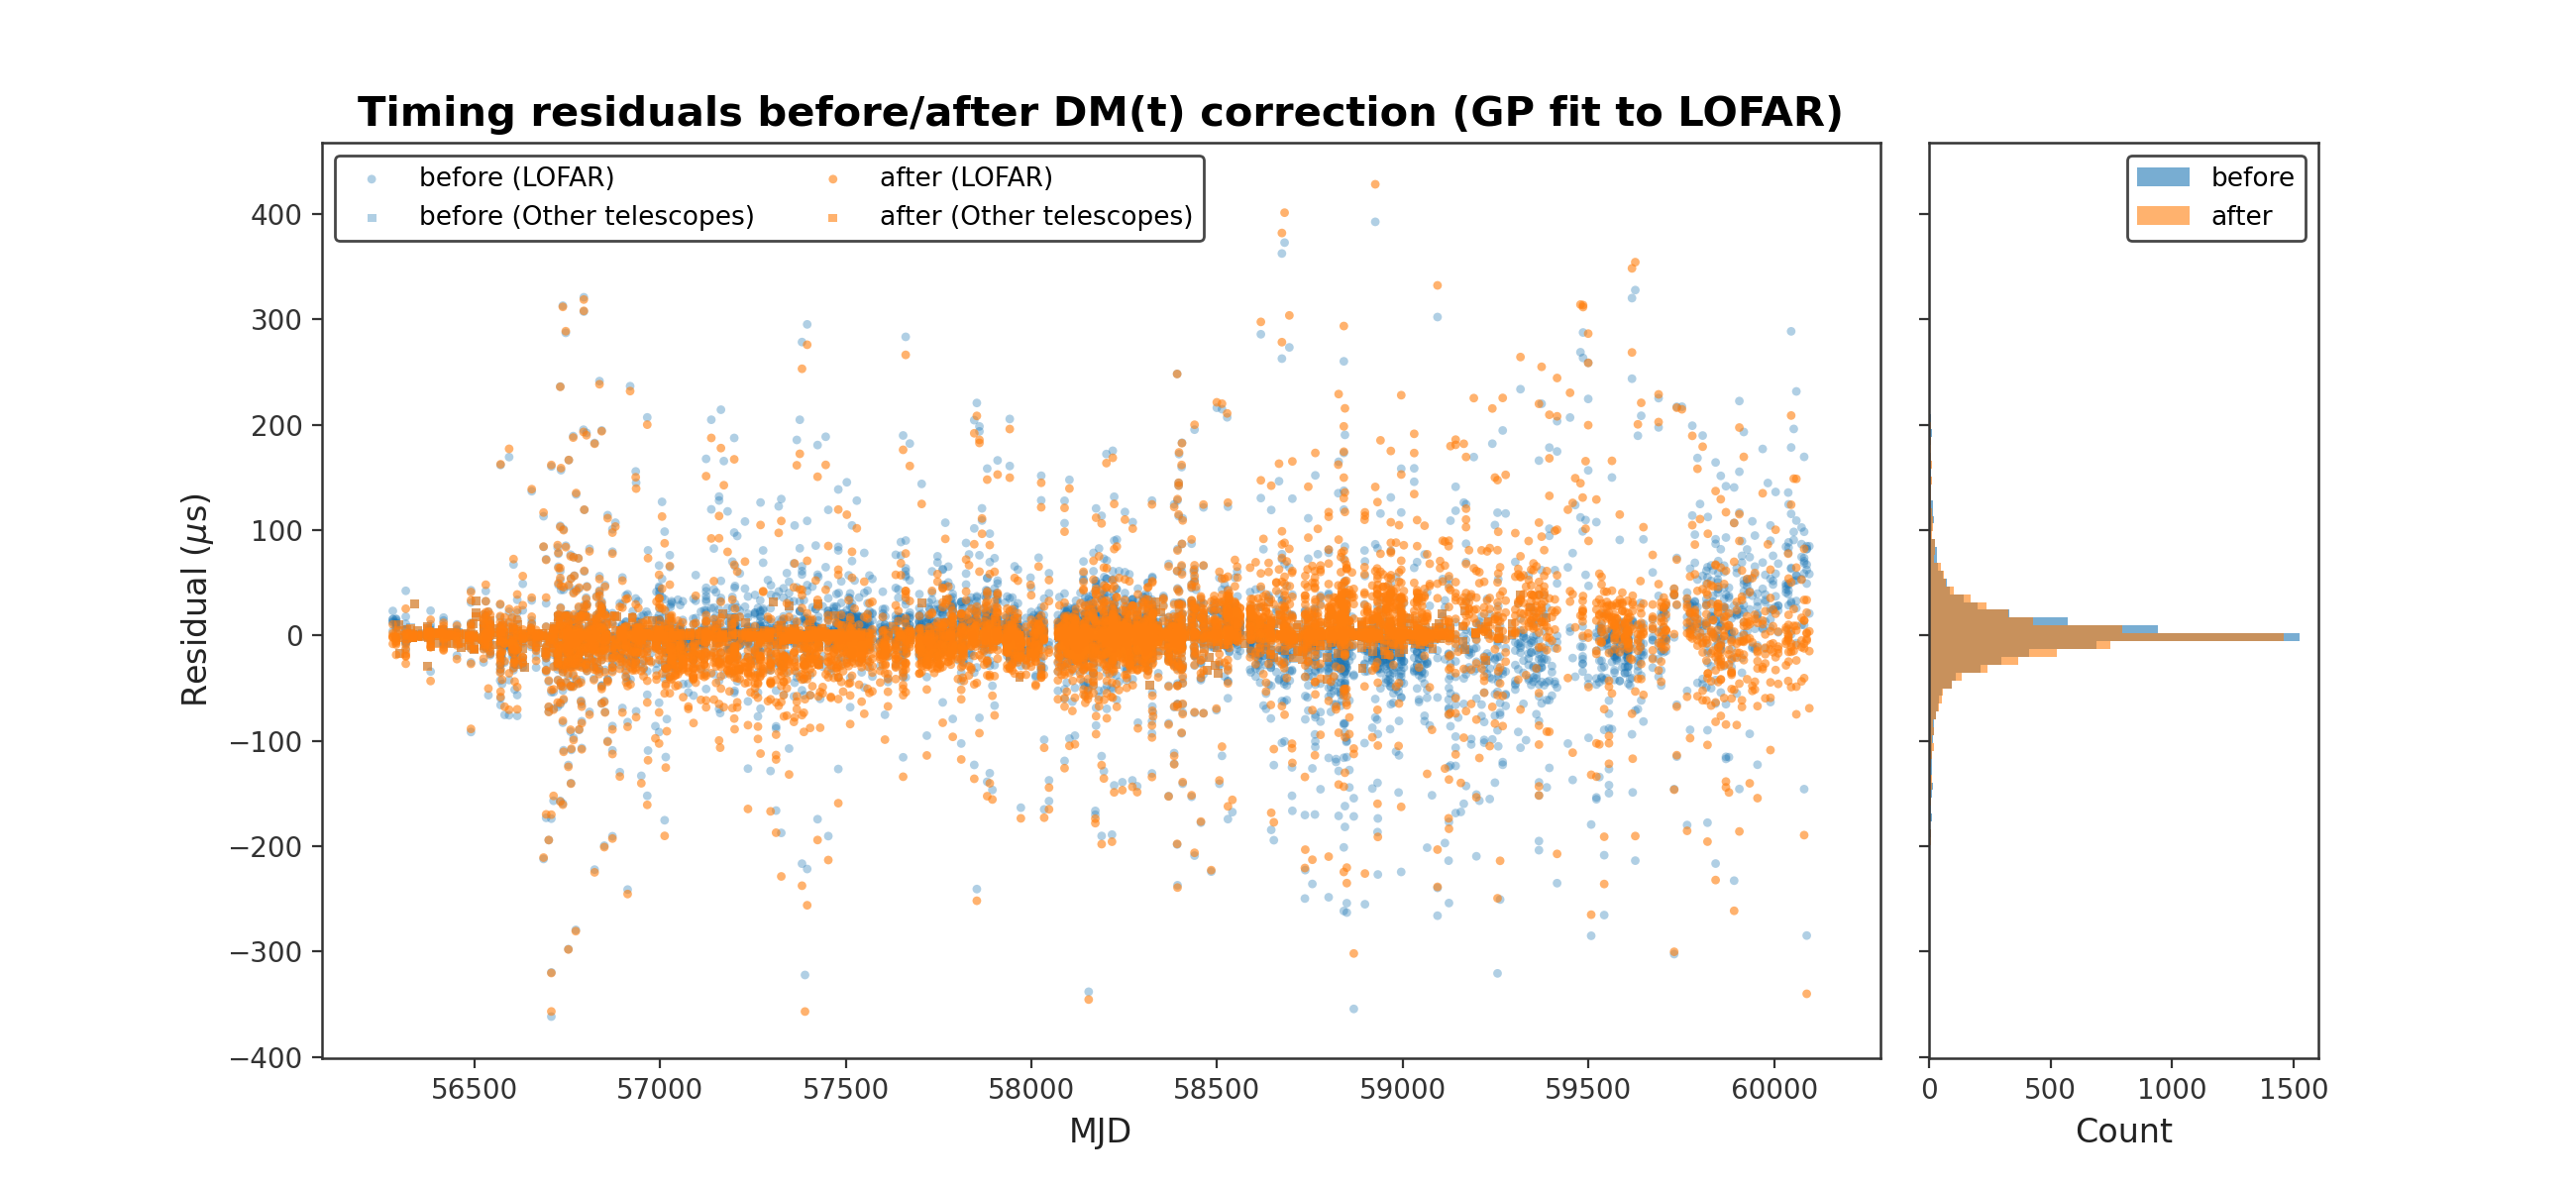
\includegraphics[width=0.8\textwidth]{../J1640+2224/dm_correction_out/residuals_pre_post.png}
\end{center}

\subsection{Noise-model comparisons}

\colorkeytable{J1640+2224}

\cmpjoint{../plot_output/compare/J1640+2224.pdf}{highfreq\_corrected: rnonly vs dmrn}
\cmpjoint{../plot_output/compare/J1640+2224_lofaronly_corrected_rnonly_vs_dmrn.pdf}{lofaronly\_corrected: rnonly vs dmrn}
\cmpjoint{../plot_output/compare/J1640+2224_corrected_dmrn_3way.pdf}{corrected, dmrn: highfreq vs lofaronly vs combined}
\cmpone{../plot_output/compare/J1640+2224_corrected_rnonly_3way.pdf}{corrected, rnonly: highfreq vs lofaronly vs combined}
\cmpjoint{../plot_output/compare/J1640+2224_uncorrected_vs_corrected.pdf}{combined: uncorrected vs corrected (dmrn)}
\cmpjoint{../plot_output/compare/J1640+2224_lofaronly_corr_vs_uncorr_dmrn.pdf}{lofaronly: corrected vs uncorrected (DM+RN)}
\cmpone{../plot_output/compare/J1640+2224_lofaronly_corr_vs_uncorr_rnonly.pdf}{lofaronly: corrected vs uncorrected (RN only)}
\cmpjoint{../plot_output/compare/J1640+2224_rnonly-corrected_vs_dmrn-uncorrected.pdf}{combined\_corrected:rnonly vs combined\_uncorrected:dmrn}
\cmpjoint{../plot_output/compare/J1640+2224_lofaronly_uncorrected_rnonly_vs_dmrn.pdf}{lofaronly\_uncorrected: rnonly vs dmrn}
\cmpone{../plot_output/compare/J1640+2224_rnonly_highfreqU_vs_lofaronlyU_vs_combinedU.pdf}{RN only, uncorrected: highfreq vs lofaronly vs combined}

\subsection{DM(t): GP reconstruction vs epoch-wise}
\cmpwide{../plot_output/compare/J1640+2224_dm_timeseries_ew_vs_gp.pdf}{combined\_corrected:dmrn DM GP vs the original epoch-wise curve}

\subsection{Interpretation}

J1640+2224 is the most informative of the three. In both
\emph{combined\_uncorrected:dmrn} and \emph{highfreq\_corrected:rnonly}, the
red-noise posterior is essentially unconstrained --- it rails against the
low-$\gamma$ edge of the prior with no clear peak, i.e.\ no real achromatic
signal is detected in either case. Yet in \emph{combined\_corrected:rnonly}
a well-determined red-noise peak appears at $\gamma\approx5$--$6$. Since
that peak only shows up once LOFAR is in the dataset \emph{and} there is no
DM GP to catch chromatic power, the most likely reading is that it is not
genuine broadband red noise but DM-like residual power leaking into the
achromatic channel --- i.e.\ the correction has not (yet) fully removed the
chromatic structure this pulsar's LOFAR data carries.

The three-way station split shows this is not simply \emph{lofaronly}'s own
signal bleeding through unchanged: under \emph{rnonly}, \emph{lofaronly}
alone finds its own well-constrained but \emph{different} peak
($\gamma\approx2$), while \emph{combined}'s peak sits at an even
\emph{higher} $\gamma$ than either sub-component on its own --- a value
neither \emph{highfreq} nor \emph{lofaronly} individually produce. Once a DM
GP is added (\emph{dmrn}), the ranking flips: \emph{combined} and
\emph{highfreq} both become essentially unconstrained, while
\emph{lofaronly}'s own red noise stays sharply peaked at
$\gamma\approx1.5$--$2$ regardless. This non-additivity --- \emph{combined}
is not a blend of its parts, and which station subset ``wins'' flips
depending on whether a DM GP is present --- is itself evidence that neither
an achromatic-only nor a DM+achromatic fit is cleanly separating genuine
broadband red noise from residual chromatic structure here. At the
\emph{lofaronly} level alone, however, the simple corrected-vs-uncorrected
comparison with no DM GP shows substantial overlap --- unlike J1012+5307 ---
suggesting the \emph{combined\_corrected:rnonly} anomaly specifically
depends on \emph{mixing} LOFAR with high-frequency stations, not on
anything intrinsic to the LOFAR band by itself. The same DM-GP reassignment
degeneracy as J1012+5307 is nonetheless present within \emph{lofaronly}
too: adding a DM GP leaves corrected red noise unchanged while uncorrected
goes fully unconstrained, with the DM GP cleanly detecting a signal
($\gamma\approx2$, well-localized) only in the uncorrected data. The
three-way \emph{rnonly} split among the three \emph{uncorrected} station
sets again gives three mutually exclusive, well-determined peaks.
